\newpage
\section{Classical Statistical Model}
Up to this point, we have acquired many statistical tools, and it is now time to step back and look at the whole picture. First, we collect a set of data points $(x_i, y_i)$. We then select an appropriate statistical model for the data, typically a parameterized one, and find the optimal parameters. Finally, we validate the model and use it to make predictions at new data points. In this section, we will discuss several statistical models. The section is organized as follows:
\begin{enumerate}
    \item Regression
    \item Classification
    \item Trees and Weak Learners
    \item Cross-Validation
    \item Time Series
\end{enumerate}

This section mainly follows STAT254 (UC Berkeley), Statistics Learning (PKU, taught by Fang Yao) and STAT153 (UC Berkeley).
I would also like to extend my heartfelt thanks to my STAT254 professor, Ryan Giordano, who has offered me countless insights and inspiration in the field of statistics.


\subsection{Regression}

\subsubsection{Fundamentals}
In general, we can define the ``loss'' of guessing $\hat{y}$ when the true value was is $y$ as
\[
\mathscr{L}(\hat{y}, y) = \mathscr{L}(f(\bx), y)
\]
We want to find $f(\cdot)$ so that $\mathscr{L}(f(\bx), y)$ is as small as possible. But the loss for a particular $f$ may depend on $\bx_{\mathrm{new}}$, since different $\bx_{\mathrm{new}}$ are associated with different distributions of $y_{\mathrm{new}}$. It follows that it doesn't make sense to minimize the loss --- instead we want to minimize the \emph{risk},
\[
\mathscr{L}(f) := \mathbb{E}\left[\mathscr{L}(f(\bx), y)\right] \qquad \text{(Risk)}.
\]
So we would like to find
\[
f^{\star}(\cdot) := \operatorname*{argmin}_{f} \mathscr{L}(f) = \operatorname*{argmin}_{f} \mathbb{E}\left[\mathscr{L}(f(\bx), y)\right].
\]

We'll consider square loss first:
\[
l(\bx, y) = \frac 1 2(y - f(\bx))^2 \quad \hat{\mathcal{L}}(f) = \frac{1}{N} \sum_{i=1}^N l(\bx_i,y_i).
\]
We cannot actually compute $f^*$, a general question is how to calculate the gap between $f^*$ and $\hat f$.
\[
0 \leq \mathscr{L}(\hat{f}) - \mathscr{L}(f^*)
= \underbrace{\mathscr{L}(\hat{f}) - \hat{\mathscr{L}}(\hat{f})}_{\text{Difficult term!}}
+ \underbrace{\hat{\mathscr{L}}(\hat{f}) - \hat{\mathscr{L}}(f^*)}_{\text{Negative term}}
+ \underbrace{\hat{\mathscr{L}}(f^*) - \mathscr{L}(f^*)}_{\text{LLN term}}.
\]
It is called generalization error and the term $\mathcal{L}(\hat f) - \hat{\mathcal{L}}(\hat f)$ can be bounded $\sup_{f} [\mathcal{L}(f) - \hat{\mathcal{L}}(f)]$, which will be discussed in the later sections.

We begin with linear regression model:
\[
y_n = \beta_1 x_{n1} + \beta_2 x_{n2} + \ldots + \beta_P x_{nP} + \varepsilon_n = \underbrace{\bx_n^\top \bbeta}_{f(\bx_n)} + \epsilon_n, \quad \text{For } n = 1, \ldots, N.
\]
where we use $N$ to denote the number of data and $P$ to denote the number of features.
To get the optimal estimator $\hat{\bbeta}$, we let
\[
0 = \frac{\partial}{\partial \bbeta} \mathcal{L}(\bbeta) \implies \bX^\top (\bY-\bX\bbeta)=0 \implies \hat{\bbeta} = (\bX^\top \bX)^{-1} \bX^\top \bY.
\]

In the general case, the optimal function is $f^*(\bx) = \EE[y \mid \bx]$, and the linear model approximates this conditional expectation as $\EE[y \mid \bx] = \bbeta^\top \bx$. To expand the function space and improve expressiveness, we sometimes apply a feature mapping to $\bx$. A simple example of a feature mapping is the polynomial mapping.
\paragraph{Splines}
For a partition $\zeta_0, \ldots, \zeta_K$ of the $x$-axis, define the indicator regressors
\[
\mathbf{z}_n^0 = \begin{pmatrix}
\mathrm{I}(\zeta_0 \leq x < \zeta_1) \\
\vdots \\
\mathrm{I}(\zeta_{K-1} \leq x < \zeta_K)
\end{pmatrix}.
\]
Regressing $y_n \sim \mathbf{z}_n^0$ produces a \emph{piecewise constant} fit, returning the average of training responses within each interval.
Indicator regressors give discontinuous fits with zero derivative. To obtain a piecewise linear fit, augment with
\[
\mathbf{z}_n^1 = \begin{pmatrix}
\mathrm{I}(\zeta_0 \leq x < \zeta_1)(x - \zeta_0) \\
\vdots \\
\mathrm{I}(\zeta_{K-1} \leq x < \zeta_K)(x - \zeta_{K-1})
\end{pmatrix}.
\]
Regressing $y_n \sim \mathbf{z}_n^0 + \mathbf{z}_n^1$ yields a separate first-order Taylor approximation within each segment.
Generalizing to degree $p$,
\[
\mathbf{z}_n^p = \begin{pmatrix}
\mathrm{I}(\zeta_0 \leq x < \zeta_1)(x - \zeta_0)^p \\
\vdots \\
\mathrm{I}(\zeta_{K-1} \leq x < \zeta_K)(x - \zeta_{K-1})^p
\end{pmatrix},
\]
gives a $p$-th order polynomial fit within each bucket.

\paragraph{Bias and Variance Trade-off}
Let’s decompose this target $\mathbb{E}\left[(\hat{f}(\mathbf{x}_{\mathrm{new}}) - y_{\mathrm{new}})^2\right]$.
\begin{align*}
\mathbb{E}\left[(\hat{f}(\mathbf{x}_{\mathrm{new}}) - y_{\mathrm{new}})^2\right]
&= \mathbb{E}\left[(\hat{f}(\mathbf{x}_{\mathrm{new}}) - \bar{f}(\mathbf{x}_{\mathrm{new}}) + \bar{f}(\mathbf{x}_{\mathrm{new}}) - f^{\star}(\mathbf{x}_{\mathrm{new}}) + f^{\star}(\mathbf{x}_{\mathrm{new}}) - y_{\mathrm{new}})^2\right] \\
&= \underbrace{\mathbb{E}\left[(\hat{f}(\mathbf{x}_{\mathrm{new}}) - \bar{f}(\mathbf{x}_{\mathrm{new}}))^2\right]}_{\text{``variance''}} + \underbrace{\mathbb{E}\left[(\bar{f}(\mathbf{x}_{\mathrm{new}}) - f^{\star}(\mathbf{x}_{\mathrm{new}}))^2\right]}_{\text{``bias''}} + \underbrace{\mathbb{E}\left[(f^{\star}(\mathbf{x}_{\mathrm{new}}) - y_{\mathrm{new}})^2\right]}_{\text{``irreducible error''}}.
\end{align*}
Define $M_{xx} = \EE [\bx^\top \bx]$ and $M_{xy} = \EE[\bx^\top y]$. Then $\bbeta = M_{xx}^{-1}M_{xy}$. By CLT,
\[
\hat{\bbeta} - \bbeta^*
= \left(\frac{1}{N} \sum_{n=1}^{N} \mathbf{x}_n \mathbf{x}_n^\top\right)^{-1} \frac{1}{N} \sum_{n=1}^{N} \mathbf{x}_n (y_n - \mathbf{x}_n^\top \mathbf{\beta}^*), \quad
\sqrt{N}(\hat{\bbeta} - \bbeta^*) \to \mathcal{N}(0, M_{xx}^{-1} U M_{xx}^{-1}),
\]
where $U := \operatorname{Cov}(\bx_n \epsilon_n)$. We have
\[
N \cdot\text{Variance} \approx \operatorname{tr}(M_{xx}^{-1/2} U M_{xx}^{-/2}) = \sigma^2\operatorname{tr}(I_P) = P\sigma^2 \implies \text{Variance} \approx \frac{P\sigma^2}{N}.
\]

\subsubsection{Ridge ($L_2$) and Lasso ($L_1$) Regression}
When $P \gg N$, $\bX^\top\bX$ is non-invertible, and the model is prone to overfitting---a common phenomenon in this regime. A simple remedy is to introduce a penalty term. We begin with the $L_2$ penalty.
\[
\mathcal{L}_{ridge}(\bbeta, \lambda) = \|\bY-\bX^\top\bbeta\|_2^2 + \lambda \|\bbeta\|_2^2 \implies \hat\bbeta_{ridge} = (\bX^\top \bX + \lambda \bI)^{-1} \bX^\top \bY.
\]
Assume $\bY = \bX^\top \bbeta^* + \bvarepsilon$ with $\mathbb{E}[\bvarepsilon] = \bzero$ and $\mathrm{Cov}(\bvarepsilon) = \sigma^2 \bI$. Let the singular value decomposition give $\bX^\top\bX = \bV \bSigma^2 \bV^\top$ with $\bSigma^2 = \mathrm{diag}(d_1, \ldots, d_P)$, so that $(\bX^\top\bX + \lambda \bI)^{-1} = \bV (\bSigma^2 + \lambda \bI)^{-1} \bV^\top$.

A direct computation gives
\[
\mathbb{E}[\hbbeta_{\text{ridge}}] - \bbeta^* = -\lambda \bV (\bSigma^2 + \lambda \bI)^{-1} \bV^\top \bbeta^*, \qquad \mathrm{Cov}(\hbbeta_{\text{ridge}}) = \sigma^2 \bV \, \mathrm{diag}\!\left(\frac{d_j}{(d_j+\lambda)^2}\right) \bV^\top,
\]
which yields
\[
\text{Bias: }\| \mathbb{E}[\hbbeta_{\text{ridge}}] - \bbeta^* \|_2^2 = \sum_{j=1}^{P} \frac{\lambda^2}{(d_j + \lambda)^2} (\bv_j^\top \bbeta^*)^2, \qquad \text{Variance: }\mathrm{tr}\,\mathrm{Cov}(\hbbeta_{\text{ridge}}) = \sigma^2 \sum_{j=1}^{P} \frac{d_j}{(d_j + \lambda)^2}.
\]
As $\lambda$ increases, the variance decreases while the bias increases.

Another choice is $L_1$ penalty, which we called LASSO,
\[
\mathcal{L}_{lasso}(\bbeta, \lambda) = \|\bY-\bX^\top\bbeta\|_2^2 + \lambda \|\bbeta\|_1.
\]
\begin{rem}
    LASSO favors \textbf{sparse} solutions, whereas Ridge spreads weight more evenly across coefficients. This makes LASSO a natural tool for variable selection: by tuning $\lambda$, one can identify the salient predictors as those with nonzero coefficients.
\end{rem}

\subsubsection{Kernel Methods}
Consider the Ridge Regression, by some Mathematics tricks
\[
\hat\bbeta_{ridge} = (\bX^\top \bX + \lambda \bI_P)^{-1} \bX^\top \bY = \bX(\bX \bX^\top + \lambda \bI_N)^{-1}  \bY.
\]
Note that we have replaced an $P\times P$ inverse with an $N\times N$ inverse, and may reduce computation (in some case). $\bX \bX^\top = (x_i^\top x_j)_{i,j}$, replace $x_i^\top x_j$ into $k(x_i,x_j)$, and we have kernel function.

\begin{defn}[Reproducing Kernel Hilbert Space]
Let $\cX$ be an arbitrary set and $\cH$ a Hilbert space of real-valued functions on $\cX$. We say $\cH$ is a \emph{reproducing kernel Hilbert space} (RKHS) if there is a kernel $k : \cX \times \cX \mapsto \mathbb{R}$ such that
\begin{itemize}
    \item $\forall x \in \cX,\ k(\cdot, x) \in \cH$.
    \item \emph{Reproducing property:} $\forall x \in \cX,\ f \in \cH,\ \langle f, k(\cdot, x) \rangle_\cH = f(x)$.
\end{itemize}
\end{defn}

For a kernel $k : \cX \times \cX \to \mathbb{R}$, we define an integral operator $\cT_k : L^2_\mu(\cX) \to L^2_\mu(\cX)$ as follows
\[
\cT_k f(x) = \mathbb{E}_{x' \sim \mu}[k(x, x') f(x')].
\]

\begin{thm}[Mercer's theorem]
Let $k$ be a continuous kernel on a \textbf{compact set} $\cX$. There exist an orthonormal basis $\{e_j\}_{j=1}^\infty$ of $L^2_\mu(\cX)$ such that $\forall x, x' \in \cX$,
\[
k(x, x') = \sum_{j=1}^{\infty} \lambda_j e_j(x) e_j(x').
\]
The convergence is uniform on $\cX \times \cX$ and absolute for each $(x, x') \in \cX \times \cX$.
\end{thm}
\begin{rem}
    From this perspective, an RKHS can be viewed as a subspace of $L_2$. The faster the eigenvalues $\lambda_j$ decay, the smaller the RKHS---and correspondingly, the smoother the functions it contains.
\end{rem}

This theorem ensures the existence of an eigendecomposition of a kernel $k$, i.e., the corresponding integral operator $\cT_k$. Note that $(\lambda_j)_{j \geq 1}$ and $(e_j)_{j \geq 1}$ are the eigenvalues and eigenfunctions of the integral operator $\cT_k$ in the sense that
\begin{itemize}
    \item $\cT_k e_j = \lambda_j e_j$, i.e., $\mathbb{E}_{x' \sim \mu}[k(x, x') e_j(x')] = \lambda_j e_j(x)$.
    \item $\langle e_i, e_j \rangle_{L^2_\mu(\cX)} = \mathbb{E}_{x \sim \mu}[e_j(x) e_i(x)] = \delta_{i,j}$.
\end{itemize}

\paragraph{Feature map.} Mercer's theorem gives a feature map for the kernel $k$. Let
\[
\Phi : \cX \to \ell^2, \qquad \Phi(x) = \left(\sqrt{\lambda_1} e_1(x), \sqrt{\lambda_2} e_2(x), \ldots, \sqrt{\lambda_j} e_j(x), \ldots\right)^\top.
\]
Then,
\[
k(x, x') = \sum_{j=1}^{\infty} \sqrt{\lambda_j} e_j(x) \sqrt{\lambda_j} e_j(x') = \langle \Phi(x), \Phi(x') \rangle_{\ell^2}.
\]

\begin{thm}[Spectral representation of RKHS]
Let $k$ be a continuous kernel on a compact set $\cX$, and $\{e_j\}$ be the orthonormal basis given in Mercer's theorem. Define
\[
\cH = \left\{ f = \sum_j a_j e_j : \sum_j \frac{a_j^2}{\lambda_j} < \infty \right\},
\]
with the inner product
\[
\left\langle \sum_j a_j e_j, \sum_j b_j e_j \right\rangle_{\cH} = \sum_j \frac{a_j b_j}{\lambda_j}.
\]
Then, $\cH$ is the RKHS $\cH_k$.
\end{thm}

\subsection{Classification}
\subsubsection{Fundamentals}
Let us now turn to classification problems. Like regression, we assume we get IID observations $z_n = (\mathbf{x}_n, y_n)$, but now with the difference that $y$ takes one of a set of unordered distinct values, which I will call $\mathcal{Y}$. The simplest case is where $y$ takes one of two values, which I will sometimes call ``binary classification''. As before, we wish to use $\mathbf{x}$ to guess what $y$ is. As we will see shortly, there are more choices to what $f$ should even be for classification than there are for regression.

Ultimately, we need a mapping $\mathbf{x} \mapsto \mathcal{Y}$, so we might take $\hat{y}(\mathbf{x}) \in \mathcal{Y}$. Necessarily, the loss function must take in two values in $\mathcal{Y}$---the guess and the truth---and return a real number. Formally, $\mathscr{L}: \mathcal{Y} \times \mathcal{Y} \mapsto \mathbb{R}$, which can be fully represented as a $|\mathcal{Y}| \times |\mathcal{Y}|$ matrix.
The simplest case of this is called ``zero--one'' loss:
\[
\mathscr{L}_{\text{ZO}}(\hat{y}, y) = \mathrm{I}(\hat{y} \neq y) = \sum_{c \in \mathcal{Y}} \mathrm{I}(\hat{y} = c)\, \mathrm{I}(y \neq c).
\]
Note that the maximizer of the zero--one loss has a closed form:
\begin{align*}
\mathbb{E}_{\mathbb{P}(\mathbf{x},y)}\left[\mathscr{L}_{\text{ZO}}(\hat{y}, y)\right]
&= \sum_{c \in \mathcal{Y}} \mathrm{I}(\hat{y} = c)\, \mathbb{E}_{\mathbb{P}(\mathbf{x},y)}\left[\mathrm{I}(y \neq c)\right] \\
&= \sum_{c \in \mathcal{Y}} \mathrm{I}(\hat{y} = c)\bigl(1 - \mathbb{P}(y = c, \mathbf{x})\bigr) \\
&= 1 - \sum_{c \in \mathcal{Y}} \mathrm{I}(\hat{y} = c)\bigl(1 - \mathbb{P}(y = c \mid \mathbf{x})\bigr)\mathbb{P}(\mathbf{x}).
\end{align*}
Since $\mathbb{P}(\mathbf{x})$ does not depend on $c$, the best choice for $\hat{y}$ is
\begin{equation*}
\hat{y}^*(\mathbf{x}) = \operatorname*{argmax}_{c \in \mathcal{Y}} \mathbb{P}(y = c \mid \mathbf{x}).
\end{equation*}

The natural generalization of zero--one loss and functions that return categories is a function that returns a probability. For binary regression with $y \in \{0, 1\}$, we can take $\pi(\mathbf{x})$ to approximate $\mathbb{P}(y = 1 \mid \mathbf{x})$, and so take $\pi: \mathbf{x} \mapsto [0, 1]$.

\paragraph{Cross Entropy Loss}
If $\pi(\mathbf{x}) \in (0, 1)$ then we can in fact use other losses. One common choice is the negative log likelihood:
\begin{align*}
\mathscr{L}_{\text{CE}}(\pi, y)
&= -\log \mathbb{P}(y \mid \pi) \\
&= -\log \pi^{y}(1 - \pi)^{1-y} \\
&= -y \log \pi - (1-y) \log(1 - \pi) \\
&= -y \log \frac{\pi}{1 - \pi} - \log(1 - \pi).
\end{align*}
This is also known as the ``cross-entropy loss,'' since the maximum likelihood estimator is also the minimizer of the Kullback--Liebler divergence.

\paragraph{Logistic Regression}
Suppose we have $f \in \mathbb{R}$. Then
\begin{equation*}
\pi(f) = \frac{\exp(f)}{1 + \exp(f)} =: \operatorname{Expit}(f).
\end{equation*}
You can readily see that $\operatorname{Expit}(f) \in (0, 1)$.
The expit function is invertible with inverse sometimes called the ``logit'':
\begin{equation*}
\operatorname{Logit}(\pi) := \log \frac{\pi}{1 - \pi}.
\end{equation*}
Note that if you plug this formula into the cross-entropy loss,
\begin{align*}
\mathscr{L}_{\text{CE}}(\operatorname{Expit}(f), y)
&= -y \operatorname{Logit}(\operatorname{Expit}(f)) + \log(1 - \operatorname{Expit}(f)) \\
&= -y f + \log\!\left(1 - \frac{\exp(f)}{1 + \exp(f)}\right) \\
&= -y f - \log(1 + \exp(f)),
\end{align*}
And if we further take $f(\mathbf{x}) = \mathbf{\beta}^{\top} \mathbf{x}$, we get
\begin{equation*}
\mathscr{L}_{\text{CE}}(\operatorname{Expit}(\mathbf{\beta}^{\top}\mathbf{x}), y) = -y \mathbf{\beta}^{\top} \mathbf{x} - \log(1 + \exp(\mathbf{\beta}^{\top}\mathbf{x})),
\end{equation*}
which is \textbf{logistic regression}.

\paragraph{Generative modeling}
We have noted that the optimal classifier takes the form of the maximum of $\mathbb{P}(y = c \mid \mathbf{x})\mathbb{P}(\mathbf{x})$. In our reasoning above we ignored $\mathbb{P}(\mathbf{x})$ since it does not depend on $c$, and modeled $\mathbb{P}(y = c \mid \mathbf{x})$, e.g.\ using the expit function and linear models.
However, we could condition in the other direction to write
\begin{equation*}
\hat{y} = \operatorname*{argmax}_{c} \mathbb{P}(y = c \mid \mathbf{x})\mathbb{P}(\mathbf{x}) = \operatorname*{argmax}_{c} \mathbb{P}(\mathbf{x} \mid y = c)\mathbb{P}(y = c).
\end{equation*}
When we have many more data than categories, $\mathbb{P}(y = c)$ is easy to estimate:
\begin{equation*}
\mathbb{P}(y = c) \approx \frac{1}{N} \sum_{n=1}^{N} \mathrm{I}(y_n = c).
\end{equation*}
We can then attempt to model the conditional density $\mathbb{P}(\mathbf{x} \mid y = c)$ by forming density estimates the sets of points $\mathcal{X}_c := \{\mathbf{x}_n : y_n = c\}$. Density estimation is difficult in high dimensions---arguably more difficult than estimating good decision boundaries---but generative modeling can be particularly effective in low dimensions, or when something special is known about the structure of $\mathbb{P}(\mathbf{x} \mid y = c)$.

Note that the estimation $\mathbb{P}(\mathbf{x} \mid y = c)$ does not admit a ready formulation as a direct minimization of classification error. Estimation of densities is typically considered an \textbf{``unsupervised learning''} problem for this reason, even though here we would use the unsupervised learning estimate in service of a supervised learning problem.

\subsubsection{Support Vector Machines}
Suppose we have binary classification data $(\mathbf{x}_1, y_1), \ldots, (\mathbf{x}_N, y_N)$, where $y_n \in \{-1, 1\}$, and we want to find a linear decision boundary:
\begin{equation*}
\hat{y}_n = \operatorname{sign}(\mathbf{x}_n^{T} \hat{\mathbf{\beta}}).
\end{equation*}
Such a vector $\hat{\mathbf{\beta}}$ would be normal to a hyperplane that separates our predictions.
Support Vector Machines add three layers on top of this:
\begin{itemize}
    \item \textbf{Regularization}: find the separating hyperplane with maximum margin.
    \item \textbf{Soft margin}: allow for margin mistakes (e.g.\ not linearly separable).
    \item \textbf{Kernel}: expressive (possibly infinite) feature mapping.
\end{itemize}

For finite data that are linearly separable, there always are infinitely many separating hyperplanes. Which one does perceptron converge to? If it does, con implicit, so let's make it implicit and ask for a particular one. As a form of regularization, we'll ask for the one with maximum margin:
\begin{equation*}
\hat{\mathbf{\beta}}_{\text{hard}} = \operatorname*{argmax}_{\|\mathbf{\beta}\|_2 = 1,\, \gamma} \gamma \quad \text{subject to} \quad y_n \mathbf{x}_n^{T} \mathbf{\beta} \geq \gamma \quad \forall n = 1, \ldots, N.
\end{equation*}
\begin{prop}
\begin{equation*}
\hat{\mathbf{\beta}}_{\text{hard}} = \operatorname*{argmin}_{\mathbf{\beta}} \|\mathbf{\beta}\|_2 \quad \text{subject to} \quad y_n \mathbf{x}_n^{T} \mathbf{\beta} \geq 1 \quad \forall n = 1, \ldots, N.
\end{equation*}
\end{prop}

\paragraph{Soft Margin SVM}
The hard margin SVM is restricted to linearly separable data. We now introduce a soft margin (linear) SVM, which trades separability with $\|\mathbf{\beta}\|_2$:
\begin{equation*}
\hat{\mathbf{\beta}}_{\text{soft}}(\lambda) = \operatorname*{argmin}_{\mathbf{\beta}} \sum_{n=1}^{N} \max(1 - y_n \mathbf{x}_n^{T} \mathbf{\beta},\, 0) + \lambda \|\mathbf{\beta}\|_2^2.
\end{equation*}
This way, we may allow classification (or margin) mistakes for the purpose of reducing $\|\mathbf{\beta}\|_2^2$. This brings us to the familiar form of minimizing loss plus penalty.

\paragraph{Connection to hard margin SVM}
To see how soft margin SVM relates to hard margin, add slack variable $\xi_n \geq \max(1 - y_n \mathbf{x}_n^{T} \mathbf{\beta},\, 0)$ and observe that
\begin{equation*}
\hat{\mathbf{\beta}}_{\text{soft}}(\lambda) = \operatorname*{argmin}_{\mathbf{\beta}} \|\mathbf{\beta}\|_2^2 + \frac{1}{\lambda} \sum_{n=1}^{N} \xi_n \quad \text{subject to} \quad y_n \mathbf{x}_n^{T} \mathbf{\beta} \geq 1 - \xi_n,\; \xi_n \geq 0 \quad \forall n = 1, \ldots, N.
\end{equation*}

We also divided by $\lambda$. From this point we may intuitively believe that, for linearly separable data, $\hat{\mathbf{\beta}}_{\text{hard}}$ is obtained as the limit of $\hat{\mathbf{\beta}}_{\text{soft}}(\lambda)$ as $\lambda \to 0^{+}$, since the slack variables $\xi_1, \ldots, \xi_N$ are pushed to zero.

\paragraph{Interpretation as penalty for margin mistakes}
The slack variable $\xi_n$ is nonzero if we make a margin mistake on $(\mathbf{x}_n, y_n)$. It is greater than one if we make a classification mistake. The sum $\sum_{n=1}^{N} \xi_n$ quantifies the total over all margin mistakes, which we can control by adjusting the penalty $\lambda$.

\paragraph{Kernels}
Using convex optimization theory, one may show that the soft margin SVM solution will satisfy
\begin{equation*}
\hat{\mathbf{\beta}}_{\text{soft}} = \sum_{n=1}^{N} \alpha_n y_n \mathbf{x}_n \quad ; \quad \text{where} \quad \alpha_n \neq 0 \text{ if and only if } y_n \mathbf{x}_n^{T} \hat{\mathbf{\beta}}_{\text{soft}} \leq 1.
\end{equation*}
If we used an expressive feature transformation $\varphi(\mathbf{x}_n) \in \mathbb{R}^{Q}$, the soft margin SVM $\hat{\mathbf{\beta}}_{\text{kernel}} \in \mathbb{R}^{Q}$ would satisfy
\begin{equation*}
\hat{\mathbf{\beta}}_{\text{kernel}} = \sum_{n=1}^{N} \alpha_n y_n \varphi(\mathbf{x}_n).
\end{equation*}
The prediction on a new observation would be
\begin{equation*}
y = \operatorname{sign}\!\left(\varphi(\mathbf{x})^{T} \hat{\mathbf{\beta}}_{\text{kernel}}\right) = \sum_{n=1}^{N} \alpha_n y_n \varphi(\mathbf{x})^{T} \varphi(\mathbf{x}_n)=: \sum_{n=1}^{N} \alpha_n y_n k(\mathbf{x},\mathbf{x}_n).
\end{equation*}

\subsection{Trees and Weak Learners}
\subsubsection{Classification and Regression Trees}
\begin{figure}[htbp]
    \centering
    \begin{subfigure}[t]{0.32\textwidth}
        \centering
        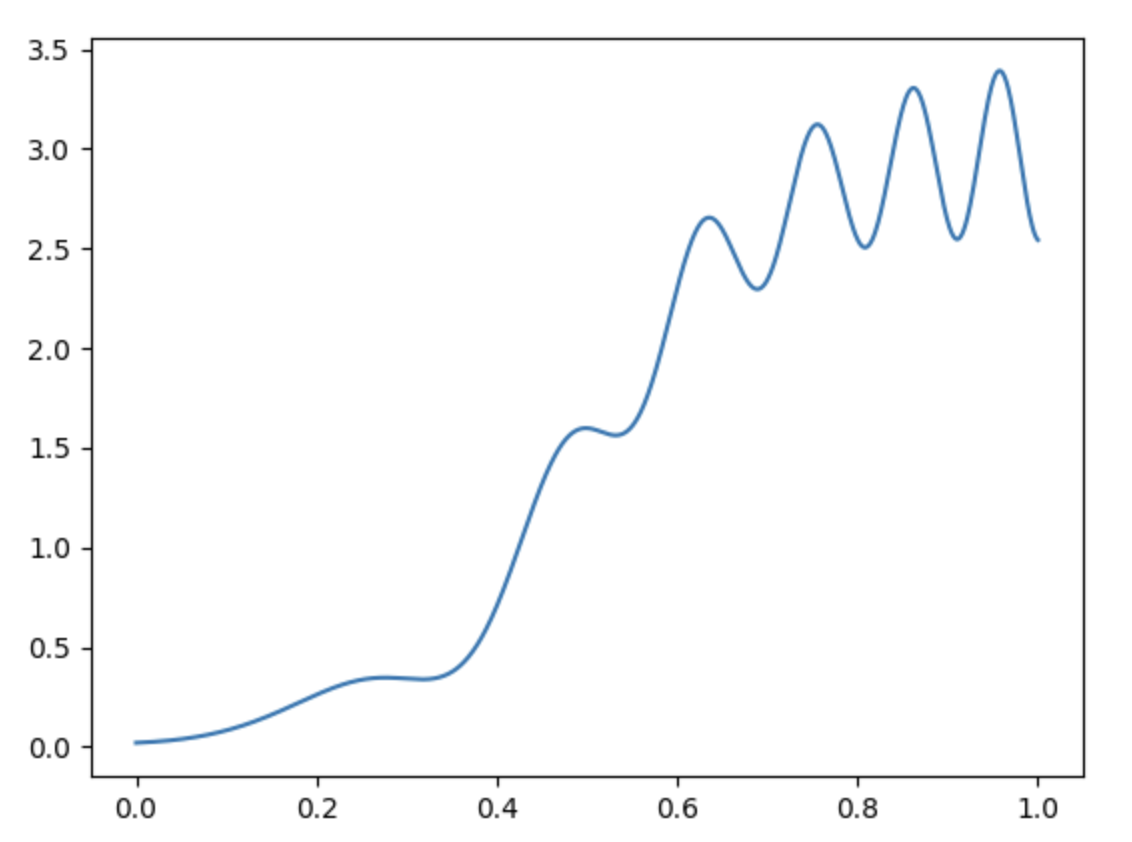
\includegraphics[width=\linewidth]{figures/CART0.png}
    \end{subfigure}\hfill%
    \begin{subfigure}[t]{0.32\textwidth}
        \centering
        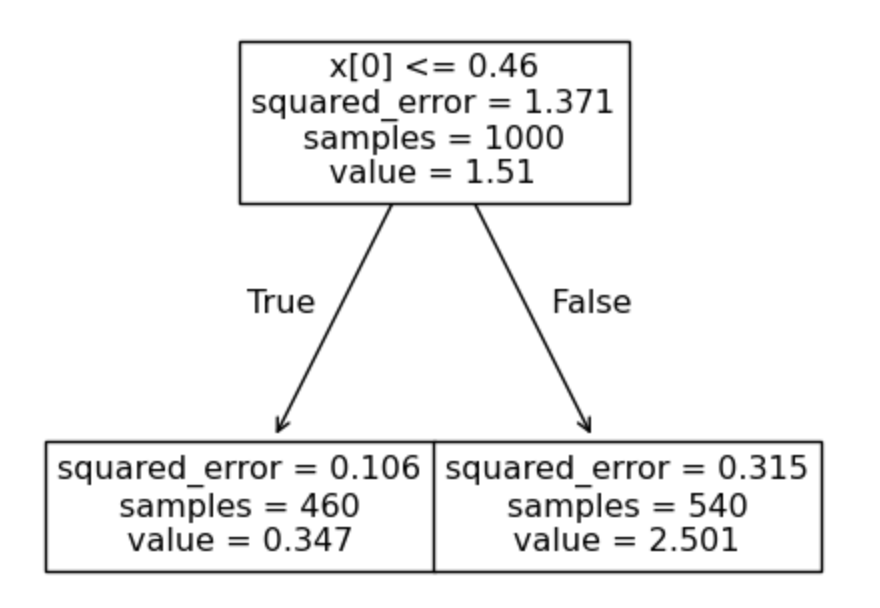
\includegraphics[width=\linewidth]{figures/TREE.png}
    \end{subfigure}\hfill%
    \begin{subfigure}[t]{0.32\textwidth}
        \centering
        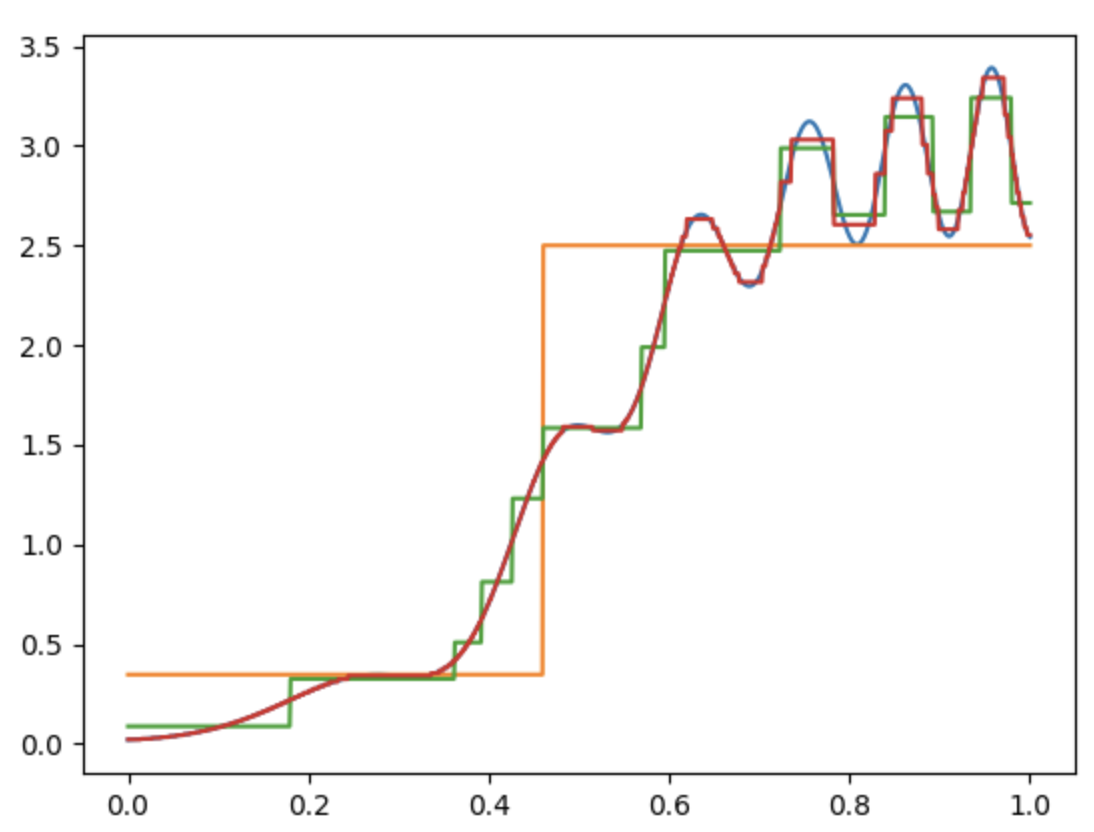
\includegraphics[width=\linewidth]{figures/CART.png}
    \end{subfigure}
    \caption{Classification and Regression Trees}
    \label{fig:cart}
\end{figure}
Classification and Regression Trees (CART) is a tree-based method that recursively splits the data into two groups based on feature values, producing a model that can predict either a category or a numerical value.

In order to choose a more optimal tree, we ``trim'' the tree back by regularizing the size of the tree. Given a starting tree $T$ and a cost complexity parameter $\alpha$, we find the subtree that minimizes
\begin{equation}
    \text{Cost complexity}\,(T') = \sum_{t \in T'} \sum_{n \in t} (y_n - \hat{y}_t)^2 + \alpha |T'|,
\end{equation}
where $t \in T'$ means $t$ is a leaf node of $T'$, $n \in t$ means $\mathbf{x}_n$ is assigned to leaf node $t$, and $|T'|$ counts the number of leaf nodes.

\subsubsection{Bootstrapping}
Let $Y_1, \ldots, Y_N$ be i.i.d.\ observations from an unknown
distribution $F$, and let $\hat{\mu} = s(\boldsymbol{Y})$ be an
estimator of a parameter $\mu$. The \emph{bootstrap} approximates
the sampling distribution of $\hat{\mu}$ by replacing $F$ with the
empirical distribution
\[
  \hat{F}(y) \;=\; \frac{1}{N}\sum_{i=1}^{N} \mathbb{I}(Y_i \le y),
\]
and resampling from the data itself. For $b = 1, \ldots, R$, draw
$\boldsymbol{Y}^{*b} = (Y_1^{*b}, \ldots, Y_N^{*b})$ \textbf{with
replacement} from $\{Y_1, \ldots, Y_N\}$ and compute the bootstrap
replicate $\hat{\mu}^{*b} = s(\boldsymbol{Y}^{*b})$. The empirical
distribution of $\{\hat{\mu}^{*1}, \ldots, \hat{\mu}^{*R}\}$ then
serves as a proxy for the sampling distribution of $\hat{\mu}$.
\begin{rem}
    Bootstrapping's power is
    computational rather than informational: it does not see more than the data, but it extracts what closed-form derivations would discard.
\end{rem}



\subsubsection{Bagging}
Suppose we're using squared error loss, and we have a learner that is
approximately \textbf{unbiased but high variance}. That is, for a particular
fixed $x$, we have $\hat{f}(x; \mathcal{D})$, where $\hat{f}(\cdot; \mathcal{D})$
depends on the training data $\mathcal{D}$, which satisfies
\[
\mathbb{E}_{\mathcal{D}}\left[\hat{f}(x; \mathcal{D})\right] \approx f^*(x)
\quad \text{and} \quad
\mathrm{Var}_{\mathcal{D}}\left(\hat{f}(x; \mathcal{D})\right) \text{ is large.}
\]
Here, $\mathbb{E}\left[y \mid x\right] = f^*(x)$ is the best possible
prediction we could make.

One might think of deep regression trees as being a possible example.
Intuitively, one might expect such a predictor to be over-fitting the
particular dataset at hand.

Recall that we showed earlier that the expected squared error decomposes into
\[
\mathbb{E}_{\mathcal{D}}\left[(\hat{f}(x; \mathcal{D}) - f^*(x))^2\right]
= \underbrace{\mathbb{E}_{\mathcal{D}}\left[\left(\hat{f}(x; \mathcal{D})
- \mathbb{E}_{\mathcal{D}}\left[\hat{f}(x; \mathcal{D})\right]\right)^2\right]}_{\text{Variance}}
+ \underbrace{\left(\mathbb{E}_{\mathcal{D}}\left[\hat{f}(x; \mathcal{D})\right]
- f^*(x)\right)^2}_{\text{Bias}}.
\]

The variance only increases the expected squared error, so if we could
get a lower-variance estimator without changing the bias, we'd improve
our loss. Ideally, we might imagine getting $B$ different, new datasets
$\mathcal{D}_1, \ldots, \mathcal{D}_B$, and then using
\[
\hat{f}_{\text{Ideal}}(x) = \frac{1}{B} \sum_{b=1}^{B} \hat{f}(x; \mathcal{D}_b)
\approx \mathbb{E}_{\mathcal{D}}\left[\hat{f}(x; \mathcal{D})\right].
\]

Of course, if we could actually do this, we should just combine the
datasets into one giant dataset. But this idea motivates the feasible
``bagging'' estimator:
\[
\hat{f}_{\text{Bagging}}(x) = \frac{1}{B} \sum_{b=1}^{B} \hat{f}(x; \mathcal{D}_b^*),
\]
where $\mathcal{D}_b^*$ is a \emph{bootstrap} sample from the original
dataset. The bootstrap distribution is a random distribution
\emph{conditional on the original dataset} $\mathcal{D}$, with probability
distribution
\[
\mathbb{P}\left((x_n^*, y_n^*) = (x_n, y_n)\right) = \frac{1}{N}
\quad \text{for} \quad n = 1, \ldots, N.
\]

The problem is, of course, that bootstrap draws are not draws from
$\mathcal{D}$. Why does bagging work? In my opinion, the theory is not
very clear, but it appears in practice that bagging tends to improve
highly variable and expressive estimators, but can make less variable
estimators worse.

\subsubsection{Boosting}
\begin{algorithm}
\caption{Forward Stagewise Additive Modeling}
\begin{algorithmic}[1]
  \State Initialize $\hat{f}_0(\cdot) = 0$.
  \For{$m = 1, \ldots, M$}
    \State Compute
      \[
        \hat{\theta}_m, \hat{\phi}_m
        \;:=\; \operatorname*{argmin}_{\theta, \phi}
        \frac{1}{N}\sum_{n=1}^{N}
        \mathcal{L}\!\left(\hat{f}_{m-1}(\boldsymbol{x}_n)
        + \theta\phi(\boldsymbol{x}_n),\, y_n\right).
      \]
    \State Set $\hat{f}_m(\cdot) = \hat{f}_{m-1}(\cdot)
      + \hat{\theta}_m \hat{\phi}_m(\cdot)$.
  \EndFor
  \State \Return $\hat{f}_M(\cdot) = \sum_{m=1}^{M}
    \hat{\theta}_m \hat{\phi}_m(\cdot)$.
\end{algorithmic}
\end{algorithm}
For boosting, we first find the $\hat{f}_1(\cdot)$ that best
predicts $y_n$, then the one that makes the biggest improvement when
added to $\hat{f}_1(\cdot)$, and so on. Note that at each step all we
need to be able to do is make a \emph{small improvement}, since over
$M$ steps these small improvements accumulate. For example, we might
take $\hat{\phi}_m(\cdot)$ to simply be a ``stump'': a regression
tree with a single split. In this sense, boosting can improve on
\textbf{high-biased estimators} by adding up a large number of them in an
\textbf{increasingly expressive} way.

\subsection{Cross-Validation}
\subsubsection{Cross-Validation}
We spend some time developing theory to control the generalization
error, $\hat{\mathcal{L}}(\hat{f}) - \mathcal{L}(\hat{f})$. In
practice, however, this theory is not useful because we cannot
actually compute the complexity. More importantly, the worst-case
bounds we computed appear in practice to be \emph{too loose} and may
suggest bad advice (see, e.g., Belkin et al.\ (2019)). In practice,
we most often \emph{estimate} the risk $\mathcal{L}(\hat{f})$ using
held-out data.

Recall that the estimator
$\hat{\mathcal{L}}(\hat{f}) = \frac{1}{N}\sum_{n=1}^{N}
\mathcal{L}(\hat{f}(\boldsymbol{x}_n), y_n)$ is not considered a
reliable estimator of $\mathcal{L}(\hat{f})$ because $\hat{f}$ is
not independent of $(\boldsymbol{x}_n, y_n)$. But suppose we have
an actual new dataset,
$\mathcal{D}_{\text{new}} = ((\boldsymbol{x}_1, y_1), \ldots,
(\boldsymbol{x}_M, y_M))$. Then we could just estimate:
\[
  \hat{\mathcal{L}}_{\text{new}}(\hat{f})
  \;\approx\; \frac{1}{M}\sum_{m=1}^{M}
  \mathcal{L}(\hat{f}(\boldsymbol{x}_m), y_m).
\]
This \emph{is} a consistent estimate of $\mathcal{L}(\hat{f})$ since
we did not use $\mathcal{D}_{\text{new}}$ to train $\hat{f}$, and so
$\hat{f}$ is independent of $\boldsymbol{x}_m, y_m$.

One might ask, if you had $\mathcal{D}_{\text{new}}$, why didn't you
just use it to train $\hat{f}$? Conversely, you might imagine taking
the data you do have, and splitting it (randomly) into a ``training
set'' $\mathcal{D}_{\text{train}}$ and a ``test set''
$\mathcal{D}_{\text{test}}$, using only $\mathcal{D}_{\text{train}}$
to compute $\hat{f}$, and $\mathcal{D}_{\text{test}}$ to estimate
$\hat{\mathcal{L}}_{\text{test}}(\hat{f})$ using the above formula.
There are costs and benefits to doing this:
\begin{itemize}
  \item You have less data to train $\hat{f}$.
  \item You have a good estimate of $\mathcal{L}(\hat{f})$.
\end{itemize}
Putting more data in $\mathcal{D}_{\text{train}}$ ameliorates the
first cost, at the risk of making your estimate of
$\mathcal{L}(\hat{f})$ worse.

A clever way to use nearly all the data to compute $\hat{f}$ and
still get a reasonable test set error is to \emph{repeat} the above
procedure many times, each time with a different test set.

As an extreme, let $\hat{f}_{-n}$ denote an estimate of $\hat{f}$
with the $n$-th datapoint removed. Since you have removed only one
datapoint, we might hope that $\hat{f}_{-n} \approx \hat{f}$, so we
have paid little estimation cost. Of course, the estimate
\[
  \hat{\mathcal{L}}_{\text{test}}(\hat{f}_{-n})
  \;=\; \mathcal{L}(\hat{f}_{-n}(\boldsymbol{x}_n), y_n)
\]
uses a single datapoint, and so is very variable, if nearly
unbiased. However, we can do this for \emph{each} datapoint and
average the results to reduce the variance of the test error
estimate. This is called the ``leave-one-out CV estimator,'' or
LOO-CV:
\[
  \hat{\mathcal{L}}_{\text{LOO}}
  \;:=\; \frac{1}{N}\sum_{n=1}^{N}
  \mathcal{L}(\hat{f}_{-n}(\boldsymbol{x}_n), y_n).
\]
Of course, you can do the same thing leaving two points out, or
three, or so on, giving ``leave-$k$-out CV'' estimators. In the
extreme where you leave a fraction $N/K$ points out, you get
``$K$-fold'' CV estimators.

How many should you leave out? There seems to be a striking lack of
useful theory. The rules of thumb are:
\begin{itemize}
  \item By leaving out more datapoints you ``bias'' your estimate
        if your estimate of $\hat{f}$ depends strongly on how many
        datapoints you have.
  \item By leaving out more datapoints you reduce the ``variance''
        of your estimate of $\mathcal{L}(\hat{f})$ by making the
        test set larger.
\end{itemize}
So there appears to be a sort of meta-bias-variance tradeoff in the
estimation of $\mathcal{L}(\hat{f})$. Common practice is five- or
ten-fold cross-validation.

\subsubsection{Influence Function}
The influence function estimates how the model parameters (or predictions)
change when a training sample is slightly perturbed, without retraining.

Let the parameters $\hat\theta$ minimize the empirical risk
$\hat\theta = \arg\min_{\theta} \frac{1}{n}\sum_{i=1}^{n} \mathcal{L}(z_i,\theta)$.
Now upweight the $i$-th sample by a small $\epsilon$, giving the perturbed
optimizer
\[
  \hat\theta_{\epsilon,z_i}
  = \arg\min_{\theta}\ \frac{1}{n}\sum_{j=1}^{n} \mathcal{L}(z_j,\theta)+\epsilon\,\mathcal{L}(z_i,\theta).
\]

Differentiating with respect to $\epsilon$ at $\epsilon=0$ yields the influence
of this sample on the parameters,
\[
  \mathcal{I}_{\text{params}}(z_i)
  = \left.\frac{d\hat\theta_{\epsilon,z_i}}{d\epsilon}\right|_{\epsilon=0}
  = -\,H_{\hat\theta}^{-1}\,\nabla_\theta \mathcal{L}(z_i,\hat\theta),
\]
where $H_{\hat\theta}=\frac{1}{n}\sum_{i=1}^{n}\nabla_\theta^2 \mathcal{L}(z_i,\hat\theta)$
is the Hessian. Since deleting a sample corresponds to $\epsilon=-\tfrac{1}{n}$,
the parameter change from removal is approximately
$-\tfrac{1}{n}\,\mathcal{I}_{\text{params}}(z_i)$.

By the chain rule, the influence of a training sample $z$ on the loss at a test
point $z_{\text{test}}$ is
\[
  \mathcal{I}(z,z_{\text{test}})
  = -\,\nabla_\theta \mathcal{L}(z_{\text{test}},\hat\theta)^{\top}\,
       H_{\hat\theta}^{-1}\,
       \nabla_\theta \mathcal{L}(z,\hat\theta).
\]
Intuitively, the more aligned the two gradients are after weighting by
$H_{\hat\theta}^{-1}$, the more the training sample $z$ helps that prediction.

\subsection{Time Series}
\todo
